\documentclass[tikz,border=10pt]{standalone}
\usepackage{tikz}
\usetikzlibrary{arrows.meta,positioning,fit,calc,backgrounds,shapes.geometric}

\begin{document}
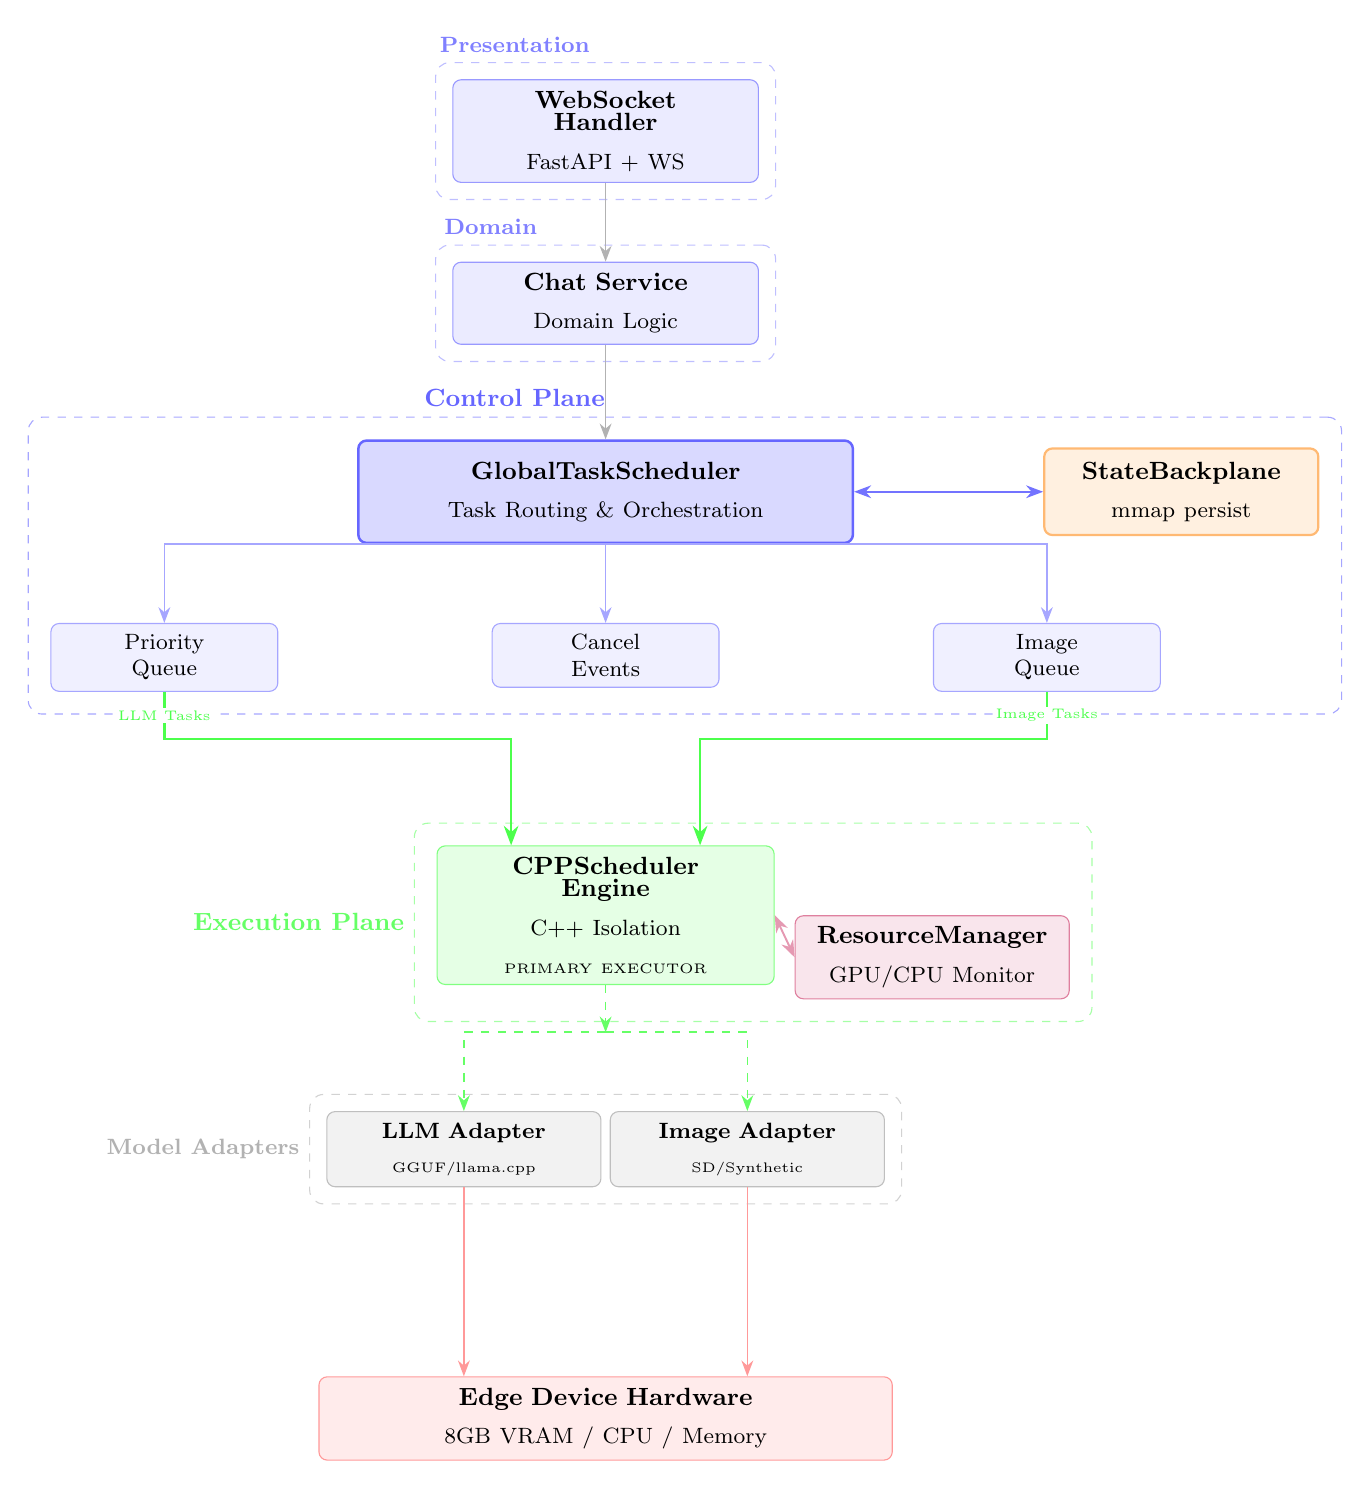
\begin{tikzpicture}[
    font=\small,
    >=Stealth,
    node distance=8mm,
    box/.style={draw, rounded corners=3pt, minimum height=9mm, align=center, inner sep=4pt, font=\small},
    layerbox/.style={box, fill=blue!8, draw=blue!40, text width=36mm, minimum height=10mm},
    corebox/.style={box, fill=blue!15, draw=blue!60, line width=0.9pt, text width=42mm, minimum height=11mm},
    subbox/.style={box, fill=blue!6, draw=blue!35, text width=26mm, minimum height=8mm, font=\footnotesize},
    execbox/.style={box, fill=green!10, draw=green!50, text width=40mm, minimum height=11mm},
    fallbackbox/.style={box, fill=yellow!10, draw=yellow!50, text width=36mm, minimum height=10mm},
    adapterbox/.style={box, fill=gray!10, draw=gray!50, text width=32mm, minimum height=9mm, font=\footnotesize},
    persistbox/.style={box, fill=orange!12, draw=orange!55, line width=0.8pt, text width=32mm, minimum height=11mm},
    resourcebox/.style={box, fill=purple!10, draw=purple!50, text width=32mm, minimum height=10mm},
    arrow/.style={->, >=Stealth, line width=0.6pt, draw=gray!60},
    doublearrow/.style={<->, >=Stealth, line width=0.7pt, draw=blue!55},
    dataarrow/.style={->, >=Stealth, line width=0.6pt, draw=green!60, dashed},
    fallbackarrow/.style={->, >=Stealth, line width=0.6pt, draw=orange!60, dotted},
    mainarrow/.style={->, >=Stealth, line width=0.9pt, draw=green!70},
]

% ==================== Presentation Layer ====================
\node[layerbox] (websocket) {\textbf{WebSocket}\\[-1mm]\textbf{Handler}\\[1mm]{\footnotesize FastAPI + WS}};

% ==================== Domain Layer ====================
\node[layerbox, below=10mm of websocket] (chatservice) {\textbf{Chat Service}\\[1mm]{\footnotesize Domain Logic}};

% ==================== Control Plane ====================
\node[corebox, below=12mm of chatservice, text width=60mm, minimum height=13mm] (scheduler) {\textbf{GlobalTaskScheduler}\\[1mm]{\footnotesize Task Routing \& Orchestration}};

% Scheduler internal components
\node[subbox, below left=10mm and 10mm of scheduler] (priority) {Priority\\Queue};
\node[subbox, below=10mm of scheduler] (cancel) {Cancel\\Events};
\node[subbox, below right=10mm and 10mm of scheduler] (imagequeue) {Image\\Queue};

% ==================== State Backplane ====================
\node[persistbox, right=24mm of scheduler] (backplane) {\textbf{StateBackplane}\\[1mm]{\footnotesize mmap persist}};

% ==================== Execution Layer ====================
\coordinate (exec-y) at ($(cancel.south) + (0,-20mm)$);

% CPPSchedulerEngine is the main executor (centered between priority and image queues)
\coordinate (cpp-x) at ($(priority.south)!0.5!(imagequeue.south)$);
\node[execbox, anchor=north, minimum height=14mm] (cppengine) at (cpp-x |- exec-y) {\textbf{CPPScheduler}\\[-1mm]\textbf{Engine}\\[1mm]{\footnotesize C++ Isolation}\\[1mm]{\tiny PRIMARY EXECUTOR}};

% ResourceManager (right side)
\node[resourcebox, anchor=north] (resource) at ($(cppengine.east) + (20mm,0)$) {\textbf{ResourceManager}\\[1mm]{\footnotesize GPU/CPU Monitor}};

% ==================== Model Adapters ====================
\coordinate (adapter-y) at ($(cppengine.south) + (0,-16mm)$);

\node[adapterbox, anchor=north] (llmadapter) at ($(cppengine.south) + (-18mm,-16mm)$) {\textbf{LLM Adapter}\\[1mm]{\tiny GGUF/llama.cpp}};

\node[adapterbox, anchor=north] (imageadapter) at ($(cppengine.south) + (18mm,-16mm)$) {\textbf{Image Adapter}\\[1mm]{\tiny SD/Synthetic}};

% ==================== Hardware Layer ====================
\node[box, fill=red!8, draw=red!40, below=12mm of cppengine, text width=70mm, minimum height=10mm] (hardware) at ($(llmadapter.south)!0.5!(imageadapter.south) + (0,-12mm)$) {\textbf{Edge Device Hardware}\\[1mm]{\footnotesize 8GB VRAM / CPU / Memory}};

% ==================== Background Frames ====================
\begin{pgfonlayer}{background}
    % Domain Layer
    \node[draw=blue!25, dashed, rounded corners=5pt, inner sep=6pt,
          fit=(chatservice),
          label={[font=\footnotesize\bfseries, text=blue!50]above left:Domain}] {};
    
    % Presentation Layer  
    \node[draw=blue!25, dashed, rounded corners=5pt, inner sep=6pt, 
          fit=(websocket),
          label={[font=\footnotesize\bfseries, text=blue!50, xshift=8mm]above left:Presentation}] {};
    
    % Control Plane - only scheduler and internal components
    \node[draw=blue!35, dashed, rounded corners=5pt, inner sep=8pt, 
          fit=(scheduler)(priority)(cancel)(imagequeue)(backplane),
          label={[font=\small\bfseries, text=blue!60, xshift=10mm]above left:Control Plane}] (cp) {};
    
    % Execution Plane - only execution components
    \node[draw=green!35, dashed, rounded corners=5pt, inner sep=8pt,
          fit=(cppengine)(resource),
          label={[font=\small\bfseries, text=green!60]left:Execution Plane}] (ep) {};
    
    % Model Adapter Layer
    \node[draw=gray!35, dashed, rounded corners=5pt, inner sep=6pt,
          fit=(llmadapter)(imageadapter),
          label={[font=\footnotesize\bfseries, text=gray!60]left:Model Adapters}] {};
\end{pgfonlayer}

% ==================== Connection Lines ====================
% Presentation -> Domain
\draw[arrow] (websocket) -- (chatservice);

% Domain -> Scheduler
\draw[arrow] (chatservice) -- (scheduler);

% Scheduler <-> State Backplane
\draw[doublearrow] (scheduler.east) -- (backplane.west);

% Scheduler -> Internal Components (stay inside control plane)
\draw[arrow, draw=blue!35] (scheduler.south) -| (priority.north);
\draw[arrow, draw=blue!35] (scheduler.south) -- (cancel.north);
\draw[arrow, draw=blue!35] (scheduler.south) -| (imagequeue.north);

% Main paths: Both queues route to CPPSchedulerEngine
% Priority Queue (LLM) -> CPPSchedulerEngine (route to left side of CPP)
\draw[mainarrow] (priority.south) -- ++(0,-6mm) -| ($(cppengine.north) + (-12mm,0)$);
\node[font=\tiny, text=green!70, fill=white, inner sep=1pt] at ($(priority.south) + (0,-3mm)$) {LLM Tasks};

% Image Queue -> CPPSchedulerEngine (route to right side of CPP)
\draw[mainarrow] (imagequeue.south) -- ++(0,-6mm) -| ($(cppengine.north) + (12mm,0)$);
\node[font=\tiny, text=green!70, fill=white, inner sep=1pt] at ($(imagequeue.south) + (0,-3mm)$) {Image Tasks};

% ResourceManager monitors CPPSchedulerEngine
\draw[doublearrow, draw=purple!40] (resource.west) -- (cppengine.east);

% CPPSchedulerEngine -> Model Adapters (cleaner routing)
\coordinate (cpp-bottom) at ($(cppengine.south) + (0,-6mm)$);
\draw[dataarrow] (cppengine.south) -- (cpp-bottom);
\draw[dataarrow] (cpp-bottom) -| (llmadapter.north);
\draw[dataarrow] (cpp-bottom) -| (imageadapter.north);

% Adapters -> Hardware
\draw[arrow, draw=red!40] (llmadapter.south) -- (hardware.north -| llmadapter.south);
\draw[arrow, draw=red!40] (imageadapter.south) -- (hardware.north -| imageadapter.south);

\end{tikzpicture}
\end{document}
